\documentclass[11pt]{article}
%
\usepackage[T1]{fontenc}
 
%
\usepackage{fullpage,amssymb,graphicx}
 
%

 \sloppy

\begin{document}
%
\title{Some illustrations of research results}

\author{Frank Nielsen\\ \ \\ Sony Computer Science Laboratories Inc.\\ Tokyo, Japan}

\date{}


\maketitle  

%ChernoffEKLInformationPDE

\begin{figure}
\centering
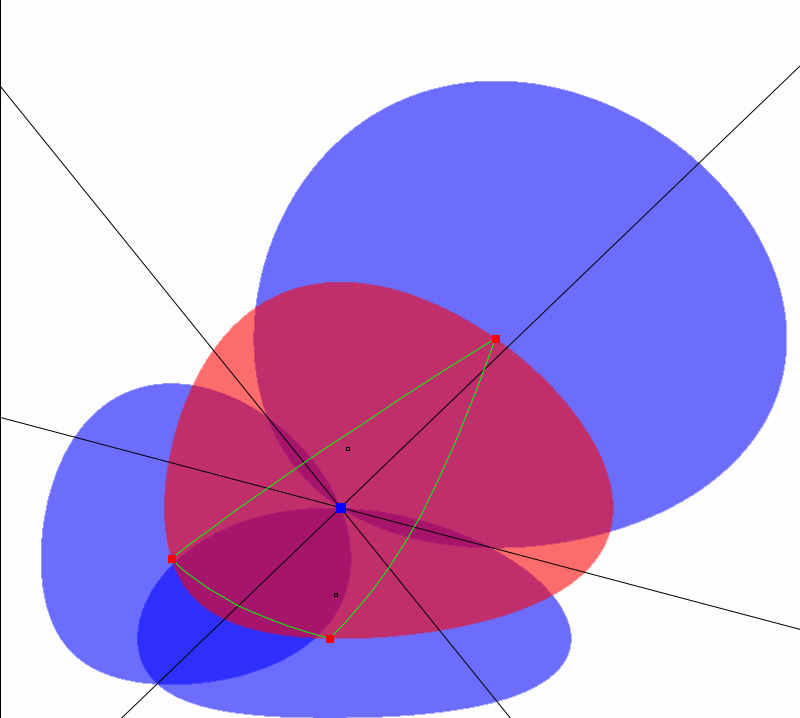
\includegraphics[width=0.5\textwidth]{eKLminiball-5pts-3pts-basis.png}

\caption{Exact smallest enclosing Bregman ball $\beta_F(\theta^*,r^*)$ (red, extended KL divergence $F(\theta)=\sum_{i=1}^2 \theta_i\log\theta_i$) of $5$ points showing $3$ basis points $\theta_1', \theta_2'$ and $\theta_3'$ (red points) on the boundary $\sigma_F(\theta^*,r^*)=\partial\beta_F(\theta^*,r^*)$.
The circumcenter $\theta^*$ (red square) is the intersection of the dual balls centered at the basis points of same radius (blue balls):
$\theta^*=\cap_{i=1}^3 \beta_F^(\theta_i,r^*)$.}\label{fig:minibball}

\end{figure}

\begin{figure}
\centering
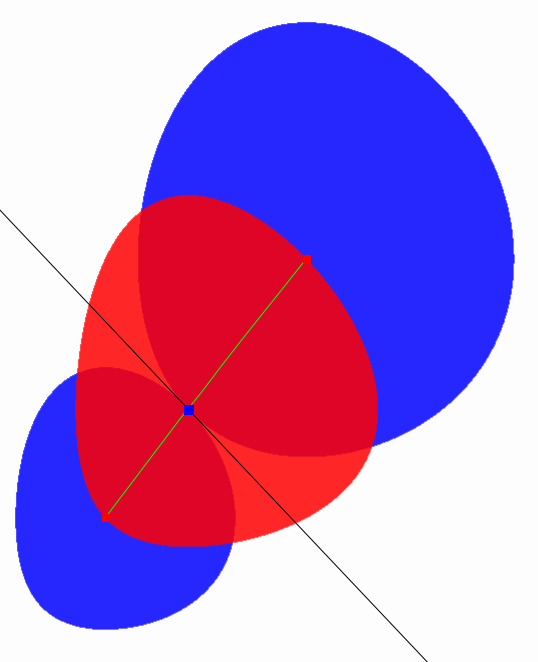
\includegraphics[width=0.5\textwidth]{ChernoffEKL-1.png}

\caption{The Chernoff information between two categorical distributions $p_{\theta_1}$ and $p_{\theta_2}$ (``trinoullis'') is the radius of the smallest enclosing ball with respect to the Bregman divergence induced by  $F(\theta)=\sum_{i=1}^2 \theta_i\log\theta_i$ (extended Shannon neg-entropy).
The circumcenter of the smallest enclosing Bregman ball is called the Chernoff point and is characterized as the intersection of the $e$-geodesic with the $m$-bisector.
 }\label{figChernoffEKL-1.png:}
\end{figure} 

%\begin{figure}
%\centering
%\includegraphics[width=]{}
%\caption{}\label{fig:}
%\end{figure}

\end{document}

\end{document}